% 独自のコマンド

% ■ アブストラクト
%  \begin{jabstract} 〜 \end{jabstract}  :日本語のアブストラクト
%  \begin{eabstract} 〜 \end{eabstract}  :英語のアブストラクト

% ■ 謝辞
%  \begin{acknowledgment} 〜 \end{acknowledgment}

% ■ 文献リスト
%  \begin{bib}[100] 〜 \end{bib}


\newif\ifjapanese

\japanesetrue  % 論文全体を日本語で書く(英語で書くならコメントアウト)

\ifjapanese
  % \documentclass[a4j,twoside,openright,11pt]{jreport} % 両面印刷の場合。余白を綴じ側に作って右起こし。 >>bindermode<<
  \documentclass[a4j,11pt]{jreport}                  % 片面印刷の場合。 >>nobindermode<<
  \renewcommand{\bibname}{参考文献}
  \newcommand{\acknowledgmentname}{謝辞}
\else
  \documentclass[a4paper,11pt]{report}
  \newcommand{\acknowledgmentname}{Acknowledgment}
\fi
\usepackage{sty/thesis}
\usepackage{ascmac}
\usepackage{graphicx}
\usepackage{multirow}
\usepackage{url}
\usepackage{here}
\bibliographystyle{jplain}

% \bindermode  % バインダー用余白設定 >>bindermode<<

% 日本語情報(必要なら)
\jclass  {卒業論文}                             % 論文種別
\jtitle    {期待和了順目の評価による\\麻雀の打牌アルゴリズムの提案}    % タイトル。改行する場合は\\を入れる
\juniv    {慶應義塾大学}                  % 大学名
\jfaculty  {環境情報学部}               % 学部、学科
\jauthor  {細田 航星}                       % 著者
\jhyear  {28}                                   % 平成○年度
\jsyear  {2016}                                 % 西暦○年度
\jkeyword  {麻雀,ゲーム情報学,AI}     % 論文のキーワード
\jproject{徳田・村井・楠本・中村・高汐・バンミーター・植原・三次・中澤・武田 合同研究プロジェクト} %プロジェクト名
\jdate{2017年1月}

% 英語情報(必要なら)
\eclass  {Bachelor's Thesis}                            % 論文種別
\etitle    {}      % タイトル。改行する場合は\\を入れる
\euniv  {Keio University}                             % 大学名
\efaculty  {Bachelor of Arts in Environmental Information}  % 学部、学科
\eauthor  {Wataru Hosoda}                           % 著者
\eyear  {2016}                                        % 西暦○年度
\ekeyword  {Mahjong, Game informatics, AI}          % 論文のキーワード
\eproject{Tokuda/Murai/Kusumoto/Nakamura/Takashio/Van Meter/Uehara/Mitsugi/Nakazawa/Takeda Labs}                 %プロジェクト名
\edate{January 2017}

\begin{document}

\ifjapanese
  \jmaketitle    % 表紙(日本語)
\else
  \emaketitle    % 表紙(英語)
\fi

% ■ アブストラクトの出力 ■
%	◆書式:
%		begin{jabstract}〜end{jabstract}	:日本語のアブストラクト
%		begin{eabstract}〜end{eabstract}	:英語のアブストラクト
%		※ 不要ならばコマンドごと消せば出力されない。

% 日本語のアブストラクト
\begin{jabstract}

ゲームAIによる昨今の成果として、囲碁や将棋などのゲームでは、人間のチャンピオンレベルの実力に至っている。一方、麻雀においては未だそれらに及んでいない。麻雀は多人数不完全情報ゲームに分類され、多人数性による複雑性と不完全情報による不確定性を理由に、適切なモデルを作成することが難しいからである。多人数性の問題では、目的の異なる相手プレイヤーの行動を予測することが難しい。また、不完全情報の問題では、未知の情報を仮定することが必要となるため、期待値による行動の決定を行わなければならない。実現可能なパターン全てを探索して比較することも、探索空間が膨大になりすぎるため非現実的である。

本研究では、以上に述べたような麻雀の性質から、問題を和了に限定し、和了率を高めるアルゴリズムに注目する。和了率は麻雀において得点する頻度を表す指標であり、これを最大化することは成績を上げるために重要である。和了率を高めるための打牌アルゴリズムとして、本研究では期待和了巡目の評価を利用する手法を提案する。期待和了巡目とは、与えられた牌姿において和了までにかかる平均消費巡目を理論値的に概算して求めたものである。これが最も小さくなるような打牌を選択することで、和了率の最大化を目指す。先行研究では単に有効牌の数だけで和了のしやすさを比較していたため、有効牌同士の優劣を精密に比較することができない問題があった。本研究の期待和了巡目を用いた手法では、有効牌をさらにブロックと呼ばれる種類ごとに分類することで、この問題を解決し、和了率を上げることを目的とする。

この手法の効果を確かめる実験として、多人数性を取り除いた1人麻雀の成績と、通常の4人麻雀の成績を、シャンテン数や有効牌を指標としたアルゴリズムや人間プレイヤーと比較した。本手法で構築したアルゴリズムは1人麻雀において、シャンテン数だけで比較するアルゴリズムよりも約10%、有効牌の数だけで比較するアルゴリズムよりも約3%高い和了率を示すことがわかった。4人麻雀では、それぞれよりわずかに和了率とレーティングが上回ったが、統計的に優位な差ではなかった。


\end{jabstract}


% 英語のアブストラクト
\begin{eabstract}

Recent achievements by game AI have led to human champion's ability in games such as Go and Shogi. On the other hand, Mahjong has not yet reached it. Mahjong is categorized as a multi-player incomplete information game, and it is difficult to create an appropriate model for reasons of complexity due to multiplicity and uncertainty due to incomplete information.

In this thesis, we propose a method to use the evaluation of expected winning cycle as batting tile algorithm to raise the rate of winning.

As an experiment to confirm the effectiveness of this method, we compare the performance of one mahjong who removed the multiplayer and the result of ordinary four person mahjong with the algorithm of related research and human player.

It was found that the algorithm constructed by this method shows higher winning rate than the algorithm to compare by merely the number of effective tiles in one person mahjong. In the 4-person mahjong, the rate of winning and ratings were slightly higher, but it was not statistically significant difference.

\end{eabstract}
  % アブストラクト。要独自コマンド、include先参照のこと

\tableofcontents  % 目次
\listoffigures    % 表目次
\listoftables     % 図目次

\pagenumbering{arabic}

\chapter{序論}
\label{chap:introduction}
\section{本論文の背景}
ゲームAIによる昨今の成果として、囲碁や将棋などのゲームでは、人間のチャンピオンレベルの実力に至っている。一方、麻雀においては未だそれに及んでいない。麻雀という競技は、多人数不完全情報ゲームに分類され、多人数性による複雑性と不完全情報による不確定性を理由に、適切なモデルを制作することが非常に難しいからである。例えば、囲碁などで利用されるゲーム木探索の手法も、以上の理由により麻雀にはそのまま適用することが出来ない。したがって、麻雀においては問題を部分ごとに取り出し、簡単な問題にしてからそれぞれを研究する必要がある。麻雀には、大きく分けて攻めと守りの戦略が存在するが、本論文では攻めの戦略について述べる。攻めの中でも、得点するために必要な和了率は非常に重要な指標であり、これを高めるための研究が数多く報告されている。和了率を高めるための研究としては大きく分けて、途中局面のヒューリスティクスを用いた方法、強者の牌譜を学習してモデルを作る方法、モンテカルロ法によるシミュレーションを用いた方法があげられる。この中で、本研究では特に途中局面のヒューリスティクスを用いた方法において、既存手法の課題を解決する手法を提案する。

\section{本論文が着目する課題}
途中局面のヒューリスティクスを用いて和了率を高めるように打牌するアルゴリズムとしては、シャンテン数を下げるように打つ方法、有効牌を最大にするように打つ方法が挙げられる。シャンテン数とは和了までの距離を表す指標で、小さいほど和了に近く、和了しやすいことを示す。したがって、与えられた牌姿14枚の中からそれぞれを打牌した場合のシャンテン数を全て計算し、最もシャンテン数が小さくなるような牌を選択するのが、最も簡単なシャンテン数を下げるように打つアルゴリズムである。しかしこの方法では、一般にシャンテン数が最も小さくなる牌は複数存在するため、その中からランダムで打牌を選択することになる。シャンテン数が最も小さくなる牌の中でも優劣は存在し、これが成績を分ける場合も多い。そのため、それらの中での優劣をつけるために一般に知られている方法が、有効牌の数を比較するという方法である。有効牌とは手牌に加えたときにシャンテン数を下げる牌の集合であり、この数が多くなるような打牌を選択することは和了率上昇につながる。しかし、この方法にはいくつかの問題点がある。一つは、有効牌の数が多いことは確かにシャンテン数を下げることを促すが、実際は有効牌にはそれぞれ種類が存在するため、数だけで比較すると正確な和了率の評価になっていない部分があることである。これは、有効牌の数が同数であっても和了率には差があることを示し、さらには有効牌の数が小さくなる選択を選んだほうが和了率が上がってしまうケースも存在することがわかっている。もう一つの問題は、この方法では目先の有効牌の数しか比較していないところである。確かに、シャンテン数を下げる牌の中から有効牌が最大になるような牌を選択することで、その瞬間次のシャンテン数を早く下げることが有利な状況になる。しかし長期的に見たときに、和了率において有利かどうかは、その瞬間の有効牌の数の比較だけではわからないことである。
% 1人麻雀においてある局面からゲーム木を展開しようとした場合、次にどの種類牌をツモるかはわからないため、ランダムに決定しノードを展開していくことになる。これを繰り返し行うと探索空間が大きくなりすぎるため、手の選択が難しくなる。これを対処するために、あらゆる手法が提案されている。このような場合に木を展開せずに有望な手を選択する手法として、Upper Confidence Bound (UCB) \cite{UCB}がある。UCB ではある局面から考えられる全ての手に対して, よい結果 を返しそうな手を重視しつつ、何度もプレイアウトと呼ば れるランダムシミュレーションを行うことで 最善の手を決定する手法である。
% UCB は局面ごとにこの探索を実行するが, 各局面を完全 に別の局面として扱うため他の局面の探索において得た情 報を利用することができない。この問題を解決するためにLinear UCB (LinUCB) \cite{LinUCB} という手法が提案されている。これは、局面を特徴で表す ことで、対象とする局面が異なっても, それまで対象とした局面の情報を利用できるといったものである。
% これらは麻雀について適用した例が報告されている\cite{LinUCB_mahjong}が、いずれの方法も平均プレイヤーに満たない成績となった。

% % しかし、UCB1 と LinUCB の評価値計算において信頼度の 計算式が異なることや、特徴量の設計に問題があるなどの理由でいい結果は出ていなかった。 
% 本研究では、モンテカルロ法の問題点である、麻雀に適用すると探索空間が大きくなりすぎてうまく適用出来ない問題に対して、探索空間を小さくするために、2つの解決策を行う。一つはモンテカルロ法のシミュレーションを直接牌姿に当てはめるのではなく、牌姿ごとの局面で数理的に比較できる内容を数理計算を用い削減する方法である。もう一つは、三向聴以下に対してはシャンテン数を下げるように打ち、モンテカルロ法を用いる部分を限定する方法である。麻雀の牌理に関しては、上がりに近づく選択ほど重要である\cite{gendai}ため、聴牌に近い打牌選択においてモンテカルロ法を適用することで、成績に影響を大きく与える部分でモンテカルロ法の効果が発揮できることが期待される。
\section{本論文の目的}
本研究では、期待和了巡目として定義する指標を用いて、和了率を高めるための打牌アルゴリズムを提案する。この手法では、与えられた牌姿におけるシャンテン数を下げる牌の中から、理論値として和了までの平均消費巡目を計算することよって、それらの牌を比較する。これにより、前節で上げた課題である、有効牌による比較アルゴリズムの問題点を解決し、和了率を改善することを目的とする。評価として、多人数性を取り除いた1人麻雀の成績と、通常の4人麻雀の成績を扱う。1人麻雀では相手プレイヤーが存在しないため、和了率を求めた打牌アルゴリズム同士の比較が精密に行えると期待できる。したがって1人麻雀では、本研究の提案手法による打牌アルゴリズムが、先に示したアルゴリズムよりも和了率として優る結果を出すことを目的とする。4人麻雀では相手プレイヤーが存在するため、和了率以外の項目でも成績に影響する要素が複雑にある。そのため、4人麻雀でも和了率が高くなることを示すことを目的とするが、その他の成績においては主に分析に利用する。
\section{本論文の構成}
本論文の構成について述べる。
\\ \ref{chap:relevantstudy}章では、ゲームAIの研究、麻雀研究の一般論について述べる。
\\ \ref{chap:approach}章では、期待和了巡目を定義し、それによって和了率を上げるための打牌を選択するアルゴリズムを提案する。
\\ \ref{chap:evaluation}章では、\ref{chap:approach}章で提案した手法で実装したアルゴリズムのAIを1人麻雀を打たせ、和了率を評価する。また、4人麻雀で打った際の成績も評価する。
\\ \ref{chap:conclusion}章では、本手法によって得られた知見について述べる。

\chapter{背景}
\label{chap:relevantstudy}

本章では不完全情報ゲームの関連研究を述べ、麻雀の関連研究の一般論について述べる。


% \section{ゲーム木探索の背景}
% 探索の方法として一般的なのは、「mini-max探索」と呼ばれているもので、自らの手はできるだけ高い評価に、そこから想定される相手の候補手はできるだけ低い評価になるように探索していく。その結果を理想的な順番に並べ、可能性の低い選択肢を切り捨てる「αβ枝刈り」を行うことで、探索を効率化させることもできる。

% ただし不完全情報ゲームにおいてはこの方法では探索空間が広がりすぎて精度を保つことが出来ないので、別の解決策を考える必要があった。

% \begin{figure}[h]
%  \centering
%  \includegraphics[keepaspectratio, scale=1.0,bb=0 0 286 215]
%       {img/minimax.png}
%  \caption{mini-max探索}
%  \label{monte2}
% \end{figure}


\section{不完全多人数情報ゲームの例}
プレイ人数に着目した研究としてはポーカーを用いたもの \cite{poker},\cite{hurui} がある。これらの手法では 2 プレイヤでのゲームを強くしてから多人数に適応する方法がとられている。ポーカーは2 プレイヤであればナッシュ均衡戦略を用いることで世界チャンピオンに勝っているが、ポーカーは 2人から 10 人程度で参加可能なゲームであり人数が増える
と状態数が指数関数的に増大するためナッシュ均衡戦略の計算は難しい。そこで 2 人で行われたナッシュ均衡戦略を3 人限定で拡張する方法、プレイヤの行動を削減、抽象化することでより少ない人数の少ないゲームを想定する方法がとられた。

\section{麻雀の例}

% 麻雀においてのAI研究については機械学習を用いた水木ら\cite{miki}や北川ら\cite{kitakawa}の研究が報告されているが、いずれも平均プレイヤの実力に至っていない。一方、水上ら\cite{bakuuti}は1人麻雀プレイ ヤの学習に牌譜との一致を目指した平均化パーセプトロンを用い、平均プレイヤ以上の実績を収めている。

% 水上らの研究より、麻雀においてもプレイヤの人数を削減してから多人数に適用する方法は有効である可能性が高く、以後ゲームを単純化した1人麻雀に対しての研究が報告されている。
% 水上ら\cite{bakuuti}1人麻雀プレイ ヤの学習に牌譜との一致を目指した平均化パーセプトロンを用いた。麻雀の特徴量は非常に膨大なため、この方法が採用された。学習に使った教師信号は、麻 雀サイト天鳳 \cite{tenhou} において鳳凰卓でプレイすることができ るプレイヤの試合データである。鳳凰卓でプレ イできるのは全プレイヤの中でも上位 0.1%程度であり牌
% 譜の質は高いと考えられる。この研究では、1人麻雀プレイヤの和了率が平均プレイヤを上回り、鳳凰卓でプレイできるプレイヤの和了率に近いレベルになった。
% しかし、1人麻雀プレイヤの学習を行う際に、4人麻雀の牌譜を使っていることで、4人麻雀独特の打ち方を排除できない問題や、上級者が認知できない最適解を求められない問題があった。


% \section{人間プレイヤーの牌譜から学習する手法を用いた研究}
% 人間プレイヤーの牌譜を教師信号とした麻雀評価関数の機械学習の報告がいくつかなされている。
% 北川らは評価関数に 3 層ニューラルネットワークを用い た教師あり学習を用いることで麻雀 AI のパラメータ調整 を行った。\cite{kitakawa}牌譜と AI の一致率はツモ局面において約56%, 鳴き局面において約89%,東風荘で得られたレートは 1318 であった[6].
% 三木らは木カーネルを用いた非線形 SVM によって手牌 の分類を学習した.ツモ局面における人間プレイヤーとの 一致率は 51%であった\cite{miki}。
% しかし、いずれの方法も人間の平均プレイヤの実力に達していない。

% 水上ら\cite{bakuuti}1人麻雀プレイ ヤの学習に牌譜との一致を目指した平均化パーセプトロンを用いた。麻雀の特徴量は非常に膨大なため、この方法が採用された。学習に使った教師信号は、麻 雀サイト天鳳 \cite{tenhou} において鳳凰卓でプレイすることができ るプレイヤの試合データである。鳳凰卓でプレ イできるのは全プレイヤの中でも上位 0.1%程度であり牌
% 譜の質は高いと考えられる。この研究では、1人麻雀プレイヤの和了率が平均プレイヤを上回り、鳳凰卓でプレイできるプレイヤの和了率に近いレベルになった。
% しかし、1人麻雀プレイヤの学習を行う際に、4人麻雀の牌譜を使っていることで、4人麻雀独特の打ち方を排除できない問題や、上級者が認知できない最適解を求められない問題があった。



\section{関連研究}
% \subsection{UCB1}
% 以上で述べたモンテカルロ法の問題点は、各ノードに対して行うシミュレーションがそれぞれ膨大なため、プレイアウトまでの回数が多く精度が落ちてしまうことである。
% この問題を解決するために、提案されている手法の中に、Upper Confidence Bound (UCB) \cite{UCB}を用いたものがある。
% UCB ではある局面から考えられる全ての手に対して, よい結果 を返しそうな手を重視しつつ、何度もプレイアウトと呼ば れるランダムシミュレーションを行うことで 最善の手を決定する手法である。有望な手に対して多くのプレイアウトを実行することで、先に述べた通常のモンテカルロ木探索よりも精度を上げることができる。以下、このアルゴリズムを詳しく説明する。

% 通常のモンテカルロ木探索では、ノードごとに期待される手の良さを途中で判定していないため、全てのノードに対して同じ回数のプレイアウトを行うことになる。したがって、良い手が期待できないノードに対しても多くのプレイアウトを割り当てることになり、無駄なシミュレーションを行ってしまう事が考えられる。また、ノードによっては手の良さを決定する分岐がプレイアウトに対して大量にある場合、他のノードと同じ回数のプレイアウトでは十分な評価が出来ない可能性もある。このような問題に対して、UCBでは、UCB1値を用いることによって各ノードの有望さをその都度確認し、全体のプレイアウトの回数や特定のノードで行われたプレイアウトの回数を考慮して、プレイアウトをどのノードに数多く割り当てるかということを判別することを考える。
% UCB1値は、${x_{j}}$は子ノード$j$の平均報酬, $α$は定数,$n$は親ノードの探索回数, ${n_{j}}$は子ノード$j$とした時、

% \begin{equation}
% \label{UCB1value}
% \Large UCB1 = \overline {x_{j}}+\alpha \sqrt {\displaystyle \frac {2\log{n}} {n_{j}}}
% \end{equation}
% で表される。
% 式 \ref{UCB1value}の右辺の第 1 項は平均報酬を, 第 2 項は信頼度を示している。従来のモンテカルロ木探索では第1項の平均報酬をそのまま全てのプレイアウトが終了するまで行った値として利用していたが、UCB1ではここで第2項の信頼度を用いることで全てのプレイアウトが終了するよりも前に信頼できる範囲を推定する。そうすることで、多くのプレイアウトを最後まで割り当てなくとも、一定の信頼度で少ないプレイアウトでそのノードが有望かどうかを判別することが可能になる。
% 信頼度はそのノードのプレイアウト回数が少ないと大きく, 多いと小さくなる。UCB1 値を用いることでUCB1 ではよ り有望そうな手に対して多くのシミュレーションを行う事 ができる。

% \begin{figure}[h]
%  \centering
%  \includegraphics[keepaspectratio, scale=0.75,bb=0 0 304 387]
%       {img/UCB.png}
%  \caption{UCBを用いたモンテカルロ木探索}
%  \label{monte2}
% \end{figure}

% \subsection{Lin UCB}
% UCB1 は各局面ごとにこの手順を実行するが, 各局面を完全に異なる局面として扱うため, 他の局面の探 索において得られた情報を共有することができないという 欠点を持つ. この欠点を補うアルゴリズムとして期待され ているのが LinUCB である.

% UCB は局面ごとにこの探索を実行するが, 各局面を完全 に別の局面として扱うため他の局面の探索において得た情 報を利用することができない。この問題を解決するためにLinear UCB (LinUCB) \cite{LinUCB} という手法が提案されている。これは、局面を特徴で表す ことで、対象とする局面が異なっても, それまで対象とした局面の情報を利用できるといったものである。

% LinUCB [5] は, UCB を局面を特徴で表すことができる ように拡張したものであり, 牌譜の局面からの教師あり学 習や異なる探索の結果の共有ができる手法である。
% LinUCB はプレイアウトを行う子ノードを選択する評価値の計算に, 重みベクトル, 特徴ベクトル, 特徴の頻度を表す相関行列を 用いる. 計算により求めた評価値が最大となる子ノードに 対してプレイアウトを行い, 共通で保持する重みベクトル を更新する. 重みベクトルは, 選択したノードの特徴ベクト ルの各項にプレイアウト結果の報酬を乗じた値を, 重みベ クトルの対応する項に足し込んで更新する. この更新によ り, 高い報酬を得た特徴は大きな重みを, 低い報酬の特徴は 小さな重みを持つようになるため, 当該ノードだけでなく, 同様の特徴を持つ他のノードの評価値も更新される. これ により異なる局面で得られた情報を共有し, 利用すること ができる. また LinUCB は探索を行った結果を重みベクト ルとして記録しておくことで, 事前学習の結果を用いる探 索として利用することも可能である.
% LinUCB のアルゴリズムを Algorithm 1 に示す. ただし xt,at はプレイアウト回数が t 回目の時の選択肢 a の特徴ベ クトル, A は特徴の共起を含めた頻度を表す相関行列, b は
% 各ノードごとの報酬の総和を表すベクトル, θt は重みベク トル, pt,a は選択肢 a の評価値, α はバランスパラメータ, rt は報酬を表している. rt はプレイアウトにより与えるか, 学習データにより与えるものとする. LinUCB は 4 行目で 前回のプレイアウト結果を反映して重みベクトル θt を更 新する. 7 行目で重みベクトル, 特徴ベクトル, 相関行列を 用いて各ノードの評価値を計算し, 9 行目で評価値が最大 となるノードを選択する. 10 行目でプレイアウトを行い報 酬を受け取り, 11 行目, 12 行目で A と b の更新を行う.
% LinUCB は Algorithm 1 の 7 行目に示したように, 式 (2) により各ノードの評価値を求める. 式 (2) の第 1 項は各ノー ドの平均報酬を計算しており, 第 2 項で信頼度を計算して いる.
% \begin{equation}
% \label{LinUCB}
% \Large pt,a = θTt xt,a + α
% \end{equation}
% また, UCB で用いている評価値も, 平均報酬と信頼度の和 で計算される. つまり LinUCB と UCB は本質的に等しい 計算をしていることが分かる. また, LinUCB の第 2 項は データ数の増加により十分速く小さくなることが保証され ている [5]. 以上より, LinUCB は UCB と近い運用を行う ことができると考えられる.

% これらは麻雀について適用した例が報告されている\cite{LinUCB_mahjong}が、いずれの方法も平均プレイヤーに満たない成績となった。

\section{本論文が着目する課題}
% 1人麻雀においてある局面からゲーム木を展開しようとした場合、次にどの種類牌をツモるかはわからないため、ランダムに決定しノードを展開していくことになる。これを繰り返し行うと探索空間が大きくなりすぎるため、手の選択が難しくなる。これを対処するために、あらゆる手法が提案されている。このような場合に木を展開せずに有望な手を選択する手法として、Upper Confidence Bound (UCB) \cite{UCB}がある。UCB ではある局面から考えられる全ての手に対して, よい結果 を返しそうな手を重視しつつ、何度もプレイアウトと呼ば れるランダムシミュレーションを行うことで 最善の手を決定する手法である。
% UCB は局面ごとにこの探索を実行するが, 各局面を完全 に別の局面として扱うため他の局面の探索において得た情 報を利用することができない。この問題を解決するためにLinear UCB (LinUCB) \cite{LinUCB} という手法が提案されている。これは、局面を特徴で表す ことで、対象とする局面が異なっても, それまで対象とした局面の情報を利用できるといったものである。以上のような対策が考えられてはいるが、1人麻雀について適用した結果平均プレイヤーの実力までに至っていない。囲碁においては一定の成果を上げたものの、麻雀ではうまく適用できない問題に対しては、麻雀の場合はより探索の空間が大きく、UCB1値やLinUCBを指標とするノードの展開の方法ではうまく適用できていない可能性がある。したがって本研究では、ノードの展開を行う際に指標とするものを麻雀というゲームの性質上の状況のパラメーターを用意し、それを使うこととする。

% しかし、UCB1 と LinUCB の評価値計算において信頼度の 計算式が異なることや、特徴量の設計に問題があるなどの理由でいい結果は出ていなかった。 
  % 本文2
\chapter{提案手法} % 一般の人がわかるレベルのアルゴリズム解説
\label{chap:approach}

本章では、以上で述べた課題に対して本研究が提案する手法を述べる。

\section{手法の概要}
本研究が提案する手法は、期待和了巡目という途中局面の静的指数を評価することで、適切な打牌を選択するアルゴリズムである。
与えられた牌姿において、和了形までにかかるツモの回数を和了までの消費巡目と定義する。ここで、麻雀においてはどのような牌をツモってくるかは確率的にしかわからず、確定的な情報ではない。したがって、和了までの消費巡目は同じ牌姿であったとしてもそれぞれの場合において異なる可能性がある。そのため、それらを十分な回数行った場合に収束することが期待される平均的な消費巡目を考える。これを、この論文では以下その牌姿における期待和了巡目とする。

\begin{figure}[h]
 \centering
 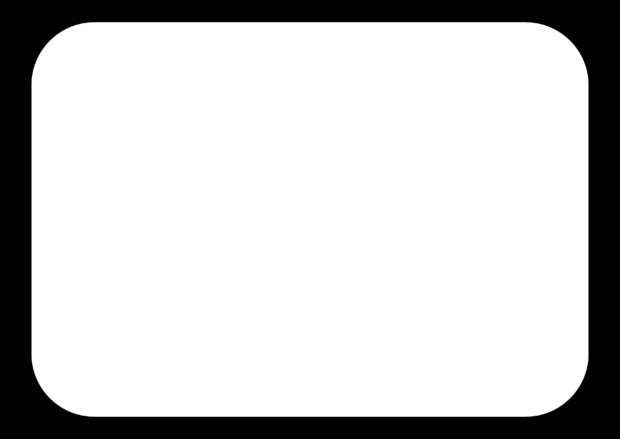
\includegraphics[keepaspectratio, scale=0.5,bb=0 0 620 439]
      {img/zu.jpg}
 \caption{期待和了巡目}
 \label{zu}
\end{figure}

\section{期待和了巡目の算出}

\subsection{変化を考慮した期待和了巡目の計算}

国士氏の研究により、ある手牌における聴牌までの平均消費順目は、それぞれの変化での平均消費巡目のそれぞれの変化する確率での単純な平均で与えられることがわかっている。[3]すなわち、図\ref{kokusi}に示すように、元の成功率がp、手変わりする確率がq,r、手変わり後の成功率がQ,Rならば、

その手の向聴が進むまでの平均消費巡目は

\begin{equation}
\label{kitai1}
\Large \displaystyle \frac {p\frac{1}{p} + q\frac{1}{Q} + r\frac{1}{R}}{p+q+r}
\end{equation}

と表される。


変化の牌姿



この式\ref{kitai1}は、他プレイヤによって捨てられた牌を使ったシャンテン数現象パターン、すなわち鳴きを考慮していない。したがって面前聴牌のみを考えた式ということになる。しかし、1人麻雀においては相手プレイヤを考慮しないため、1人麻雀における聴牌率は4人麻雀における面前聴牌確率と一致し、この式によって求まる。鳴きによって聴牌する有効牌については、全て面前ツモで聴牌する有効牌の一部であり、制限によって鳴くことが出来ない有効牌も多く存在する。例えば、以下のような牌姿の場合である。


ヘッドレスイーシャンテンの牌姿を見て解説
図


また、面前聴牌と鳴きによる聴牌の違いについては、麻雀の役の性質上、和了することができなくなる制約や、点数が下がるなどの問題がある。したがって、鳴くことによる聴牌が面前聴牌に与える影響は少ないと考えられる。

ここで、本論文ではこれを和了時までの式に拡張する。

まず平均の関係から

\begin{figure}[h]
 \centering
 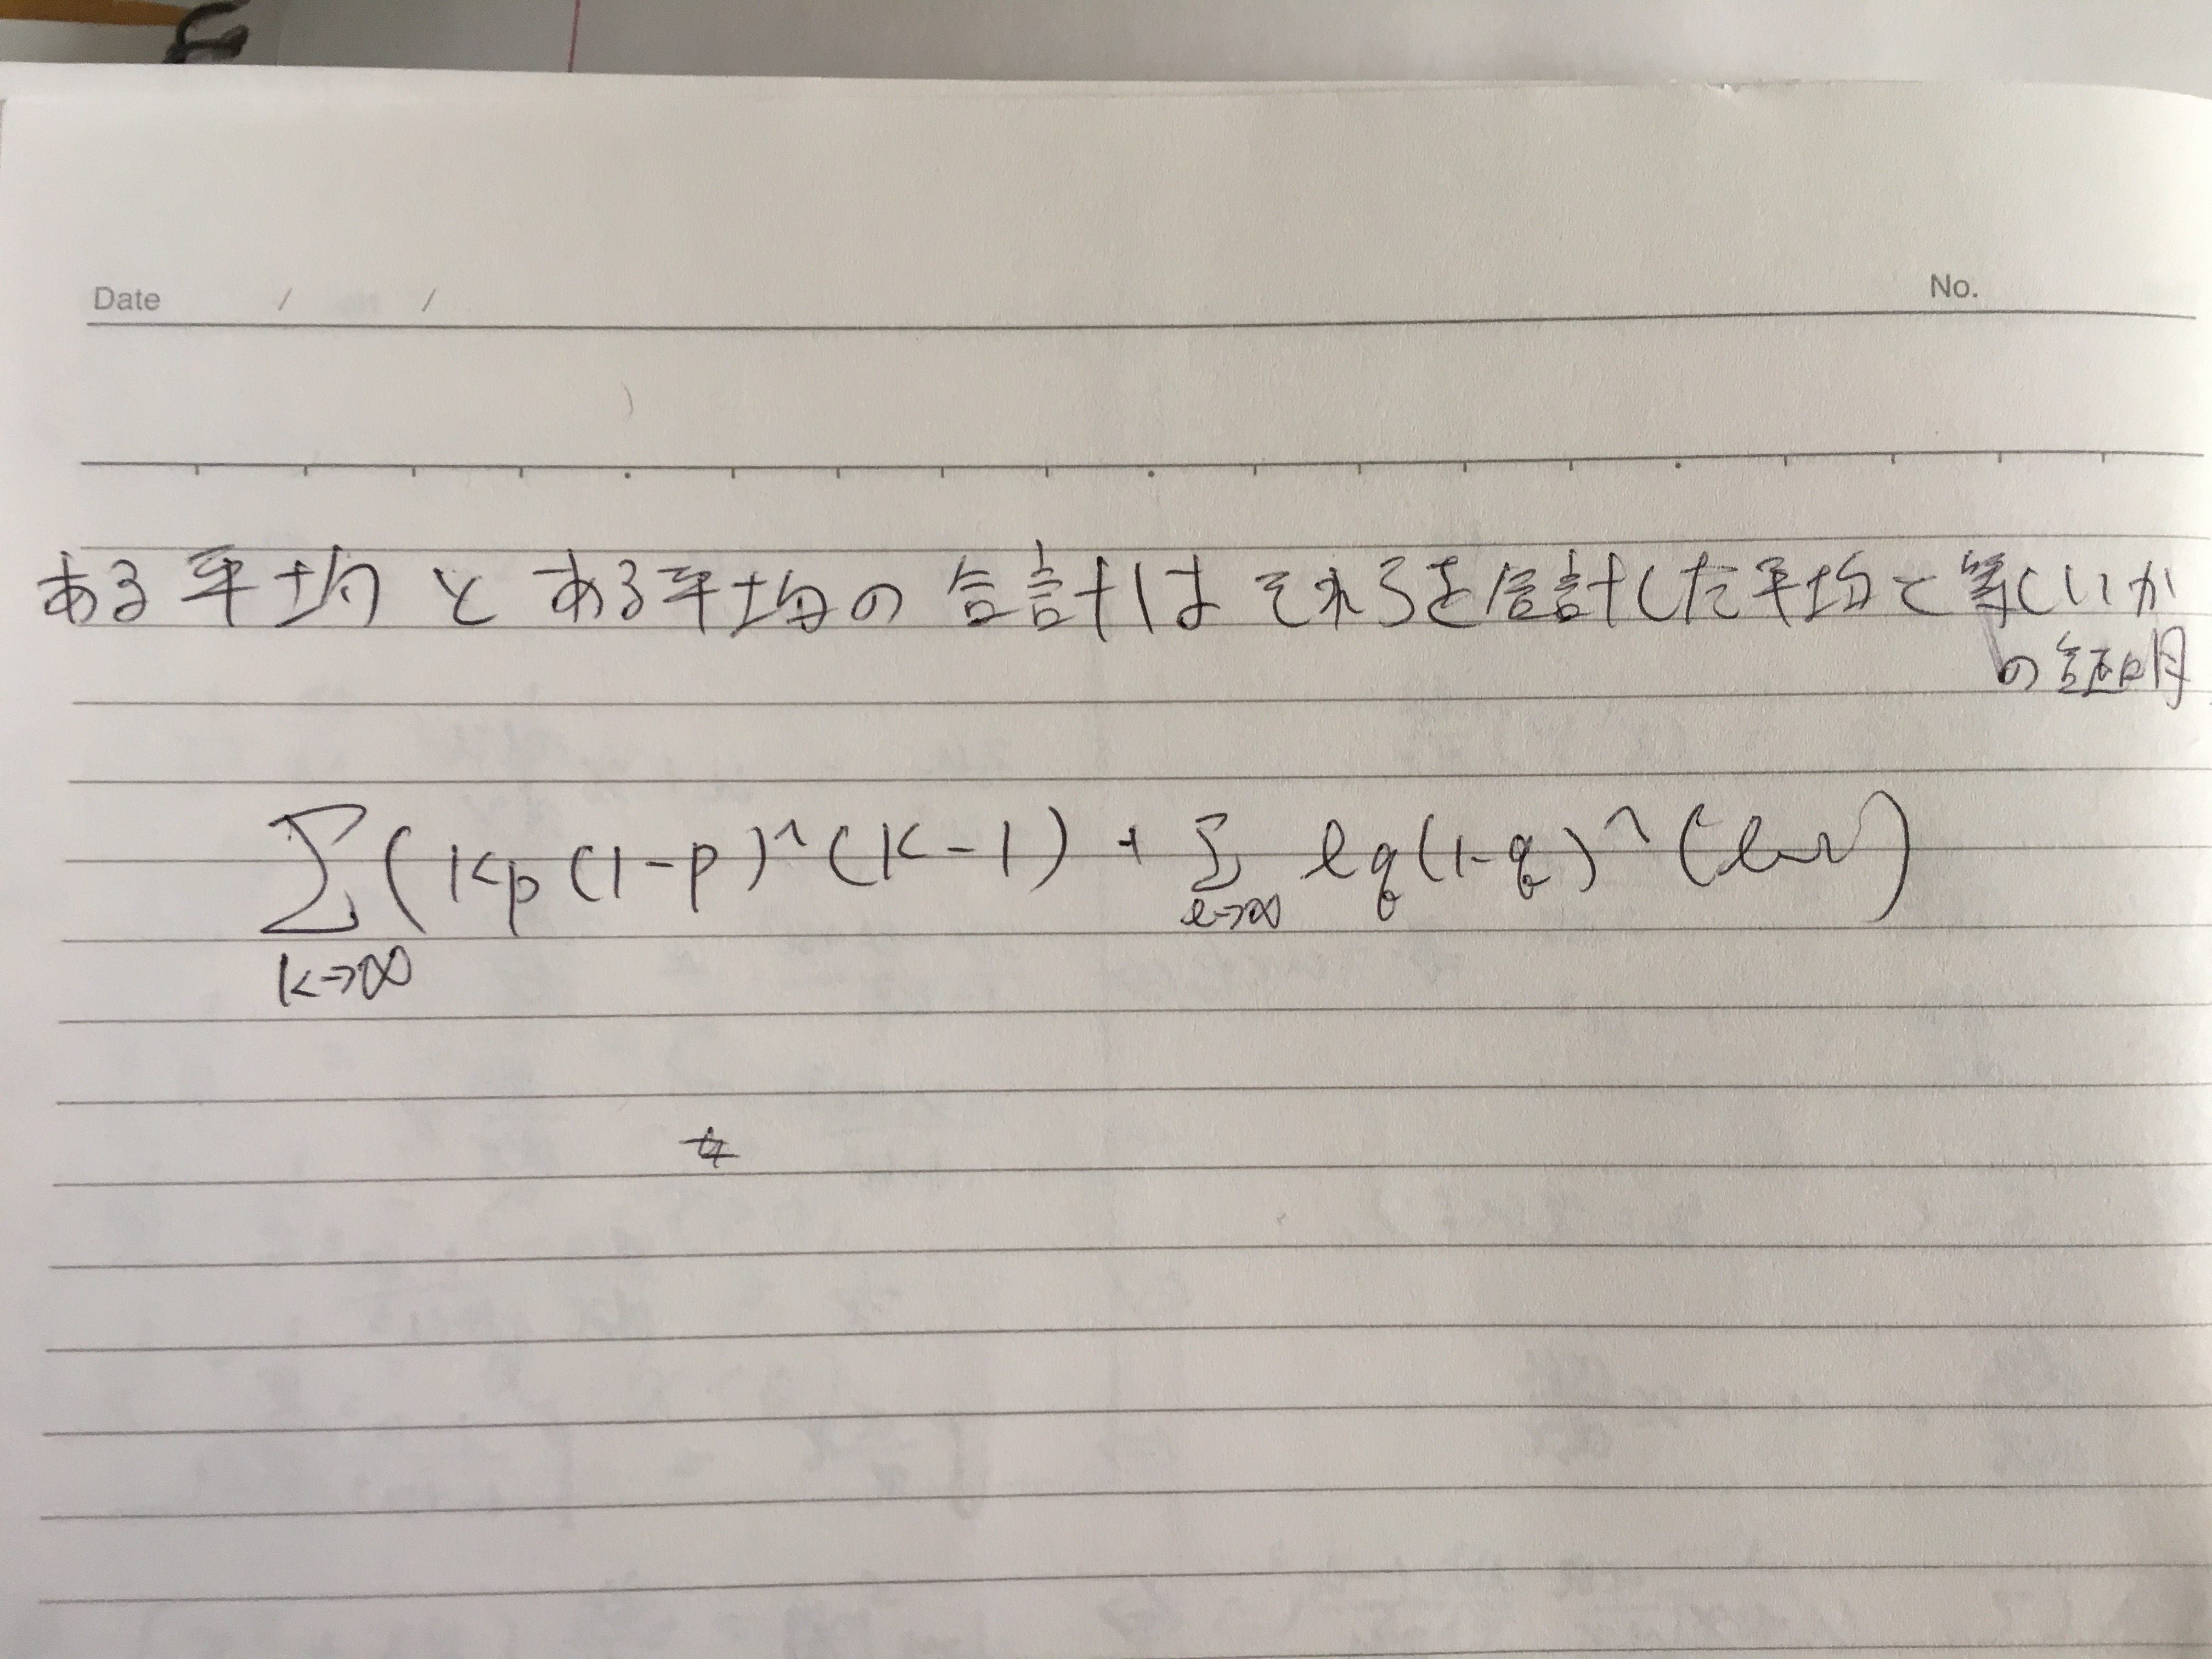
\includegraphics[keepaspectratio, scale=0.1,bb=0 0 4032 3024]
      {img/math.jpg}
 \caption{}
 \label{math}
\end{figure}

\begin{equation}
\label{kitai2}
\Large \displaystyle \frac {p\frac{1}{p} + q\frac{1}{Q} + r\frac{1}{R}}{p+q+r}
\end{equation}


ここで和了期待順目について考える


前節と同様に、4人麻雀において聴牌した

面前で聴牌するための平均消費順目と鳴きを考慮

まず、聴牌までの平均順目と聴牌後の和了までの平均順目の合計がすなわち全体の平均消費順目であることを証明する。
次に、それを合成した結果の数式がどうなるかを書く。

考察の結果このようになる。

\begin{equation}
\label{kitai2}
\Large \displaystyle \frac {p\frac{1}{p} + q\frac{1}{Q} + r\frac{1}{R}}{p+q+r} + 和了期待順目
\end{equation}
また、(現在の平均テンパイ巡目)=(次巡の平均テンパイ巡目)+1 であることから、
各ノードが手替わり率とテンパイ率を値として持つ深さ1の木構造で記述できる。 
したがって、同様に、n手先の手替わりまで考えると深さnの木構造で記述することができる。
nを大きくすることにより、精度の高い和了率を近似することが可能となる。

\begin{figure}[h]
 \centering
 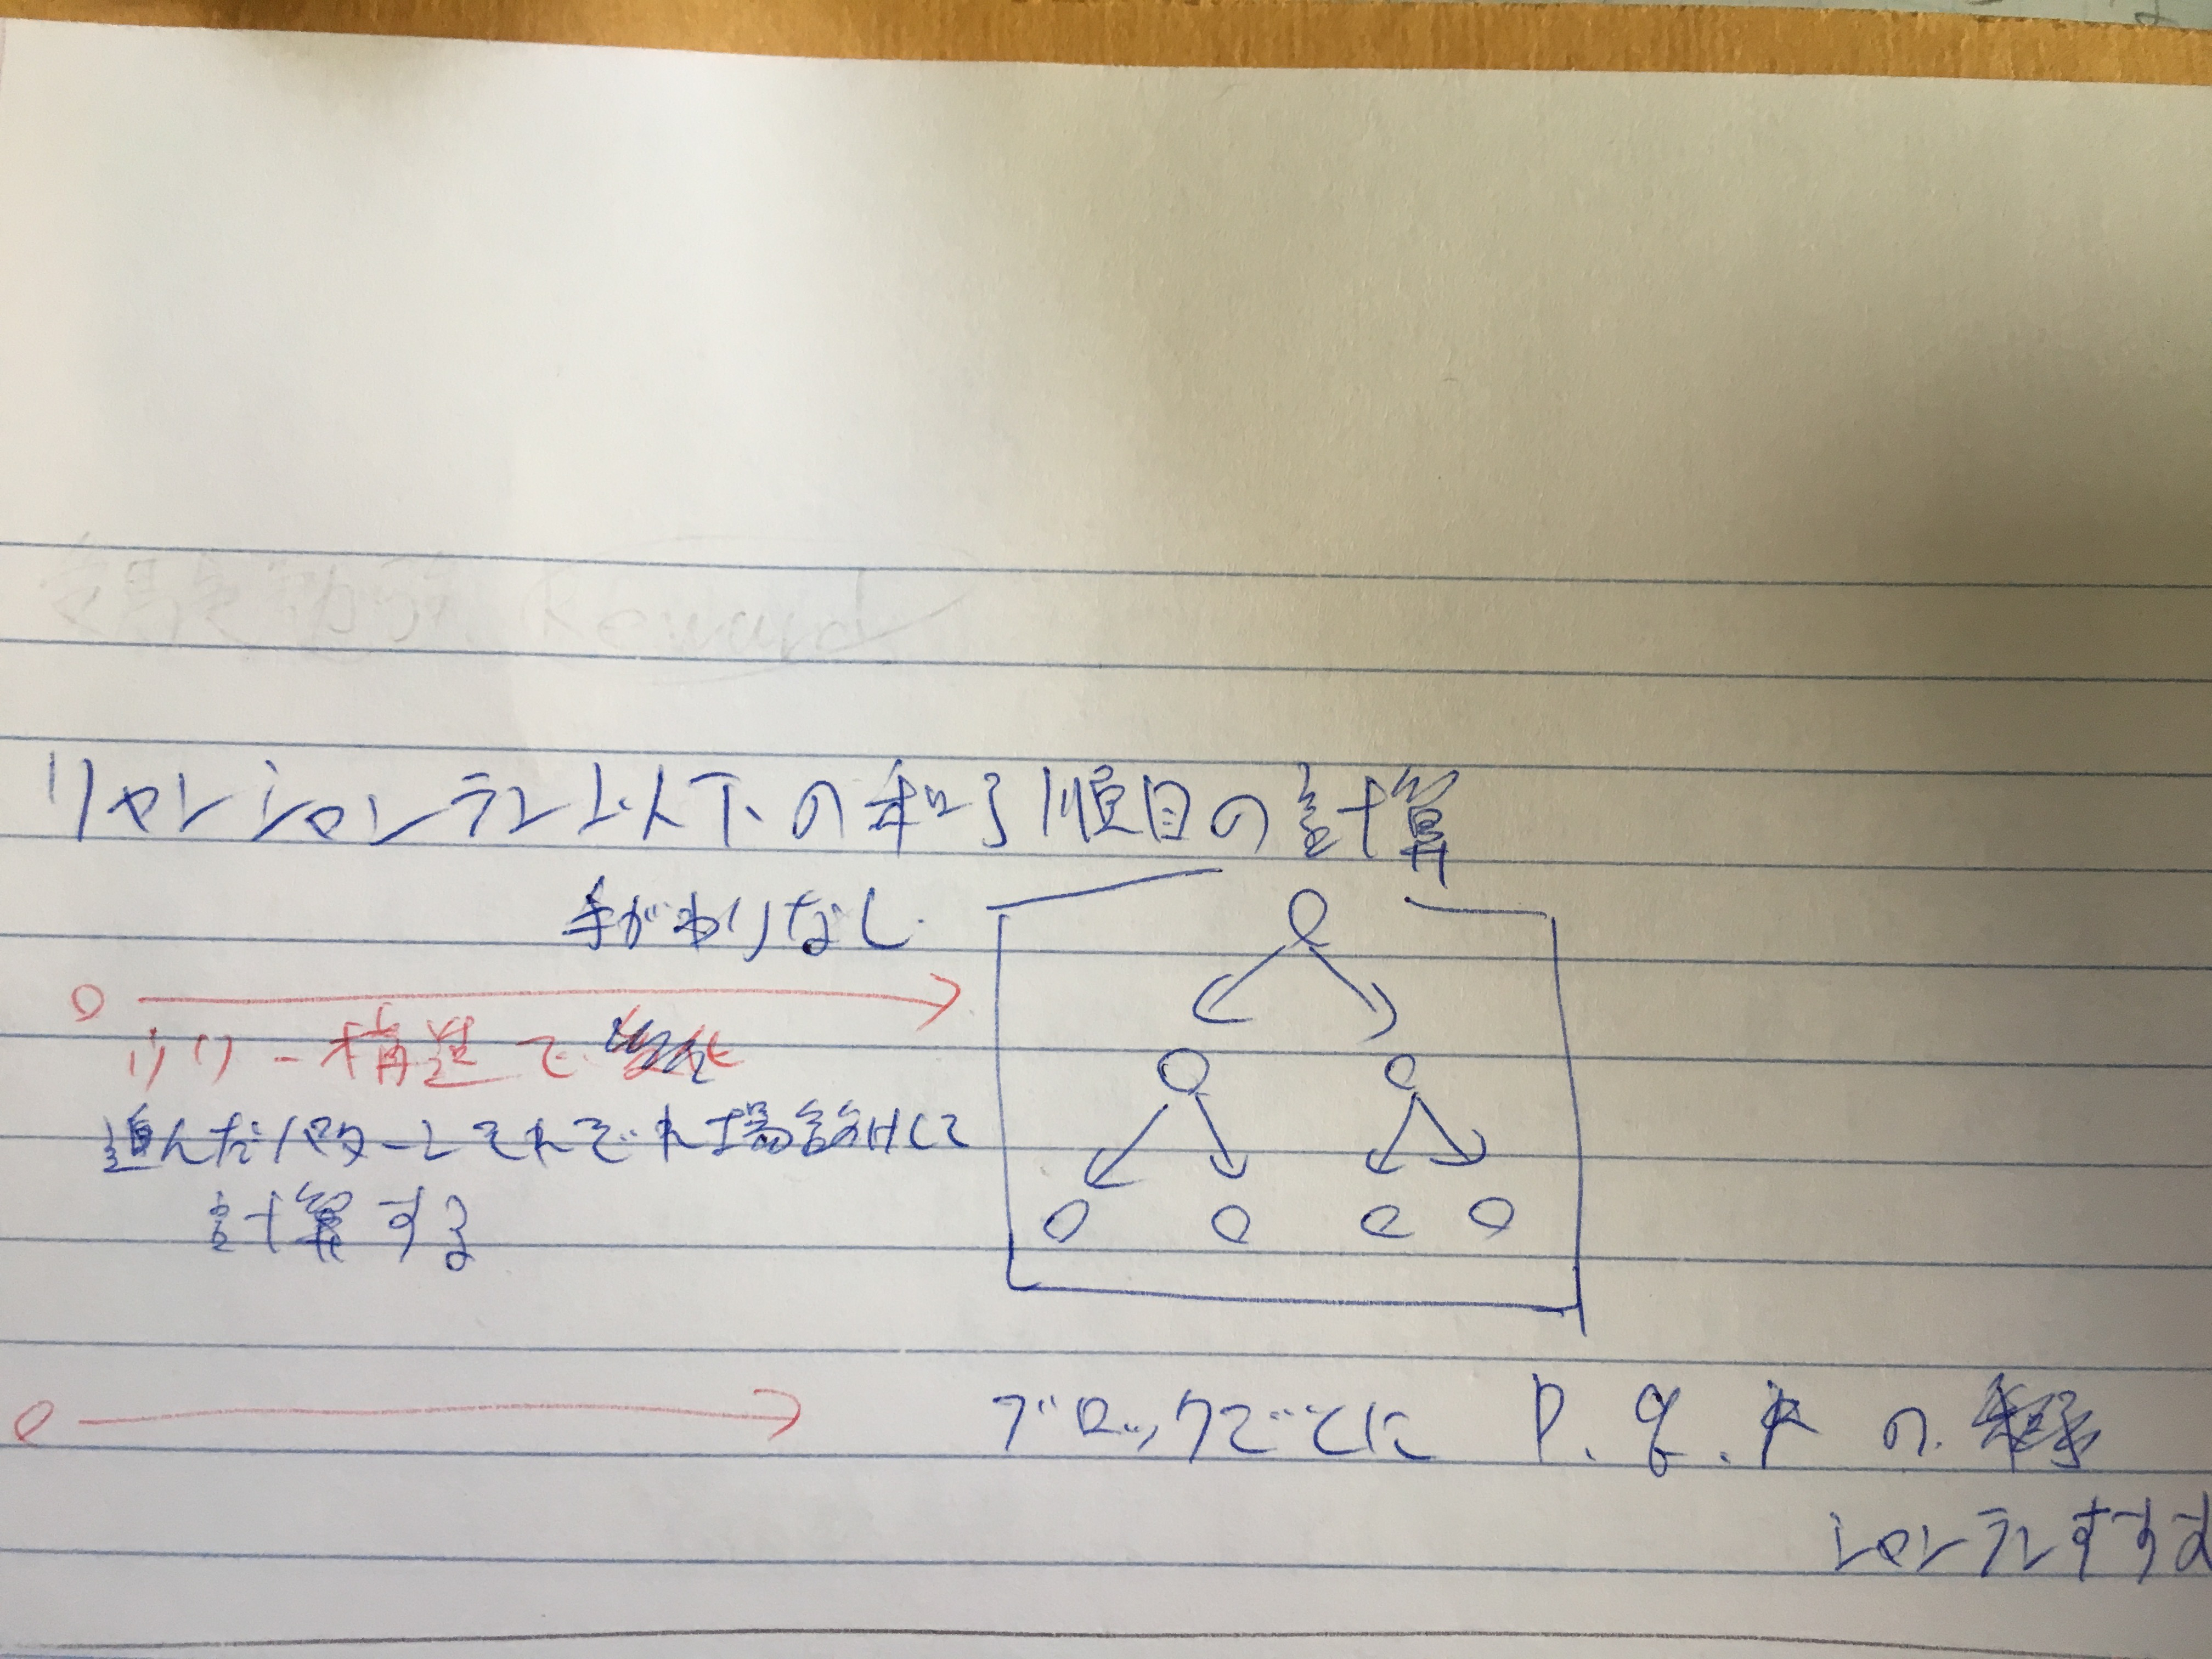
\includegraphics[keepaspectratio, scale=0.1,bb=0 0 4032 3024]
      {img/pqr.jpg}
 \caption{}
 \label{math}
\end{figure}

本研究では、この式(3)をそれぞれの牌姿に当てはめ、その計算結果が高くなるようなノードを探索する。
これにより、従来の手法では何回も同じ牌姿の変化をシミュレートしなければいけない問題があったが、(3)式の評価によってその多くが削減できる。
したがって、この方法によって精度が高くなることが期待される。





\section{想定されるメリット}
この節では、以上に提案した手法を関連研究の事例を交えて、優位性があると期待される部分について述べる。
まず最初に本手法と同じく与えられた牌姿に対して途中局面の静的指数を評価することで妥当である牌姿を選択するアルゴリズムを挙げる。これらは、モンテカルロ法などのシミュレーションをプレイアウトまで行わないものである。また、関連研究としては本手法と同じく期待和了巡目と近い考え方を用いた例を述べる。しかし、この例では期待和了巡目の算出にモンテカルロ法によるシミュレーションを使っており、静的な評価方法ではない。また、期待和了巡目の算出方法も、ツモったあとに切らないという考え方を使っており、正確な評価ではない点がある。


\subsection{シャンテン数を下げるアルゴリズムとの比較}
麻雀において、特定の和了までに必要な牌の数がシャンテン数であるため、与えられた牌姿においてのシャンテン数を把握することは和了のしやすさを評価することにつながる。これは最も基本的な方法であるため、あらゆる麻雀AIの研究で基礎として行われている。三木ら\ref{mikiUCT}は、UCTアルゴリズムの評価を行う際に、グリーディングプレイヤーとして、シャンテン数を下げるように打つプレイヤーを用いている。このグリーディングプレイヤーでは、与えられた牌姿の中で打つことのできる全ての牌に対して、打った後のシャンテン数を調べる。その後、元の牌姿とそれらのシャンテン数をそれぞれ比較し、シャンテン数が小さくなるような手を選択するアルゴリズムである。シャンテン数が同じように小さくなる手が複数あった場合には、ランダムでその中から選んだものを選択するようになっている。

\begin{figure}[h]
 \centering
 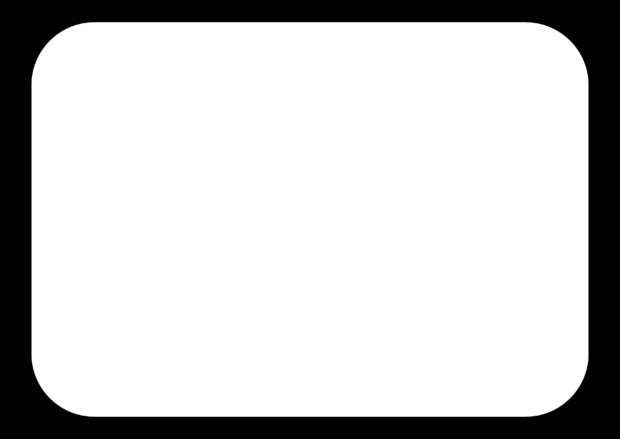
\includegraphics[keepaspectratio, scale=0.5,bb=0 0 620 439]
      {img/zu.jpg}
 \caption{シャンテン数下げるように打つアルゴリズム}
 \label{zu}
\end{figure}

この手法の問題点は〜
この代わりとしては有効牌を数えるという手が挙げられる

\subsection{有効牌の数を数えるアルゴリズムとの比較}
・有効牌の方法
・数え上げ論文の紹介

\begin{figure}[h]
 \centering
 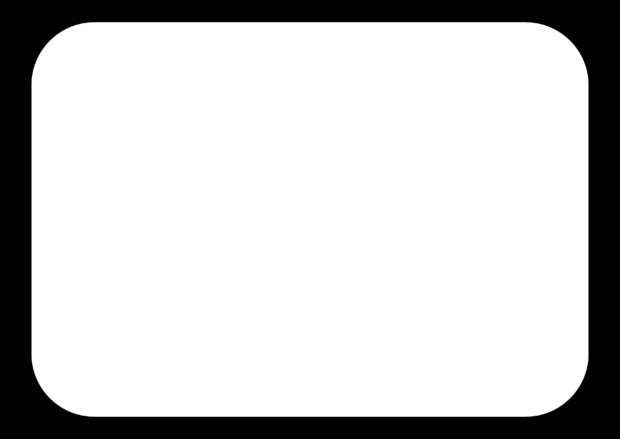
\includegraphics[keepaspectratio, scale=0.5,bb=0 0 620 439]
      {img/zu.jpg}
 \caption{シャンテン数下げるように打つアルゴリズム}
 \label{zu}
\end{figure}

この手法の問題点


\subsection{擬似的に期待和了巡目をモンテカルロ法で行った研究との比較}
期待和了巡目
シミュレーション


\section{想定されるデメリット}


% \section{和了率の評価によるノードの展開}

% 本研究では、モンテカルロ法の探索空間が大きくなりすぎる問題に対して、特定のノードの牌姿に対する期待和了順目を次の節で説明する数理モデルを使って有望だと思われる手を探索するようにする。
% 1人麻雀において特定の牌姿の期待和了順目を途中で評価できることは、より有望な手を探索できる可能性がつながるため、UCB1などの評価値よりも手の有望さを評価する精度を上げることができると期待される。

% ・期待和了順目の計算式とその証明
% ・ノード構造でできることの解説
% ・ノードをどこまで探索した方がいいかということについて
% →シャンテン数がでかすぎる場合は期待和了順目の精度が落ちること
% ・そのため、シャンテン数のでかすぎる場合についてはシャンテン数が下がる選択(有効牌は数える)
% →てかそれはそもそもそのままシャンテン数が上がる確率で求めているだけでは?
% →シャンテン数が進む場合の平均消費順目を計算しているだけ
% 期待和了巡目としても計算は可能では?実質同じっぽい。ただどこまで変化を入れるか。目先の変化だとびみょい。

% 期待和了巡目もそもそも実質有効牌を数え上げているだけだから(ただし、一巡進んだ後に排除しなければいけない有効牌を覗かないといけない。)
% これをシャンテン数がでかすぎる場合に当てはめても可能といえば可能。
% ただ当然精度が落ちる。が、そもそも有効牌を数え上げて切っているアルゴリズム自体がやってることが同じなので、これをこのまま当てはめれば多分行ける。
% 理論上は可能な気がする。

% \begin{figure}[h]
%  \centering
%  \includegraphics[keepaspectratio, scale=0.5,bb=0 0 304 387]
%       {img/UCB.png}
%  \caption{和了率評価を用いたモンテカルロ木探索}
%  \label{monte2}
% \end{figure}



% \subsection{プレイアウトと平均報酬}

% \begin{figure}[h]
%  \centering
%  \includegraphics[keepaspectratio, scale=0.1,bb=0 0 4032 3024]
%       {img/playout.jpg}
%  \caption{}
%  \label{math}
% \end{figure}

% 普通に展開した場合は平均報酬と期待和了巡目の関連性がないので、そこが問題。
% 単純に期待和了巡目で比較するか、そもそも期待和了巡目を報酬とすることで書き換えていくか。

% \subsection{二向聴以下の牌姿に対してモンテカルロ法を適用する}

% 麻雀において、和了までの手順の中では、シャンテン数が小さい時点での選択が成績に影響を与えやすいことがわかっている\cite{gendai}
% したがって、成績向上のためには和了系に近い部分において戦略を改善することが成績に影響を与えやすい事がわかる。

% また、モンテカルロ法の問題点は、前述したとおり麻雀に適用すると探索空間が大きくなりすぎることが問題であった。しかしこれを和了系に近い部分に適用することで、
% 探索空間を小さく削減することができるため、適用することができるようになる。
% 本研究の手法である与えられた牌姿における和了率の近似式(3)を適用する際にも、シャンテン数が大きすぎる場合については正確に見積もることが難しいため、このような限定的な部分への適用が重要である。

% 本論文では二向聴以上の部分にこのモンテカルロ法を適用することで、従来の問題点を解決する。
  % 本文3
\chapter{設計と実装}
\label{chap:implementation}
\section{1人麻雀の実装}
提案手法で提示した、期待和了平均順目の評価によるモンテカルロ木探索を評価するために、1人麻雀プレイヤーを実装した。
1人麻雀プレイヤーとは、相手プレイヤーを考えない多人数性を排除した麻雀のことである。ルールについては次の節で詳しく説明している。
本研究で実装した1人麻雀プレイヤーのフローチャート図を図\ref{1flow}に示す。

\begin{figure}[H]
 \centering
 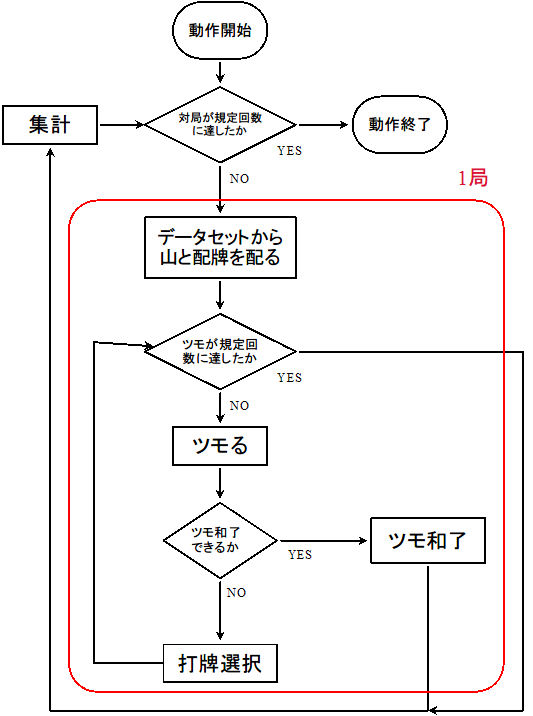
\includegraphics[keepaspectratio, scale=0.7,bb=0 0 440 540]
      {img/1flow.png}
 \caption{1人麻雀のフローチャート}
 \label{1flow}
\end{figure}

まず、1人麻雀プレイヤーにおいて開局から、終局まで行う対局のループを定義する。
開局時には、山と配牌を設置する。その後山から一つ牌をツモり、一つ捨てる動作を繰り返す。終了条件を満たした時点で終局となり、その局の成績を集計する。このループを1人麻雀プレイヤーにおける1対局と定義する。この対局のループを十分な回数行い、和了率を測定する。

% 期待和了平均順目をn順先の変化まで評価することによって性能が変わる可能性があるので、1順、2順、3順までの変化を考慮するものをそれぞれ分けて実験した。
% それぞれに対して100局のテストデータと10,000局のテストデータを与え、あがることができた局数を計測した。テストデータとは、全ての牌をランダムに並べたものを100セット用意したデータである。このデータから 13 牌を初期牌として 与え, その後牌を引いて切る動作を 27 回行い, その中であ がれたかどうかを確認した。100 局のテストデータで人間 のプレイヤとの比較を行い, 10,000 局のテストデータで各 手法の性能の評価を行った。



\subsection{1人麻雀のルール}
通常の4人麻雀では、多人数製の問題があるため、分岐や考慮すべき問題が多い難しさがある。この難しさを解消するために、相手を考慮しない1人麻雀を考える。
この1人麻雀のルールは、相手プレイヤーを考えないため、点数を支払う事による放銃や被ツモ失点などを考えない。また、相手プレイヤーによる捨て牌が存在しないので、鳴きや栄和を考えない。リーチについても、和了率の観点では不要なため、考えない。門前でツモを繰り返し行うだけのシンプルなシステムである。
% 先行研究\cite{zentsu}評価を合わせるため、ツモの回数は27回とした。

\begin{table}[htbp]
  \caption{本研究の1人麻雀プレイヤのルール}
  \label{tb:bakuuti_score}
  \begin{center}
  \begin{tabular}{c|c|c}
    \hline
    アクション  & 4人麻雀 & 1人麻雀 \\\hline\hline
    和了  & ツモ和了、ロン和了どちらも可 & ツモ和了のみ\\\hline
    点数 & 失点や和了の点数を考慮する & 点数は考えない\\\hline
    リーチ & 可能 & なし\\\hline
    鳴き & チー、ポン、カンが可能 & なし\\\hline
    終局 & 誰かが和了するか、ツモ山70枚がなくなるまで(136-14-13*4) & 和了するか、27回ツモるか\\\hline
  \end{tabular}\end{center}
\end{table}

また1人麻雀の成績の評価においてはその点数の推移よりも、和了率自体が重要だと考えられている。したがって、点数という複雑なパラメータを省いた和了率に注目したルールとなっている。その理由としては、以下のような理由が述べられる。

4人麻雀では平均順位の低いプレイヤーほど、平均和了点低く、和了率が高いことというデーターが存在する。\cite{kagaku}。したがって強いプレイヤーは点数よりも和了率を重視して打っていることがわかる。
上手いプレイヤーは手役を無理に狙わないため、平均和了点が低くなると考えられる。また麻雀の点数の特性上、満貫までの点数は指数関数的にその得点が増えていくが、満貫以上の場合は線形に近くなる。したがって、難易度に対して望める点数が割に合わない高い和了を狙うより、比較的低い点数で゙多く和了することが効率が良い。
また、失点の観点からも、4人麻雀では自分が放銃をしない場合も他プレイヤーの和了によって被ツモ失点を被ることがある。これに対しても、和了すれば他プレイヤーが和了することができないため、相手の和了を防ぐという意味でも和了率の高さは重要である。

\subsection{終了条件}
図\ref{1flow}に示した1局の終了条件は、ツモが規定回数に達するか、和了したかのいずれかとしている。4人麻雀においても、いずれかのプレイヤーが和了しない場合において、ツモの回数が規定回数(厳密には山がなくなるまでだが)に達した場合は終了となる。したがって、1人麻雀においても、和了が発生しない場合においても対局が終了するような条件を入れた。また、通常の4人麻雀ではツモの回数は、流局した場合平均的に18回である。しかし1人麻雀を評価として利用している関連研究の多く\cite{zentsu}\cite{bakuuti2013}が、1人麻雀のツモの規定回数を27回としているため、本研究でもツモの回数を27回とした。また、対局数に関しては、5000局のものと100局のもので分けた。詳しくは次章の評価で述べるが、AIアルゴリズム同士では十分な回数行い、人間プレイヤーも評価に加える際は実現が可能な100局という対局数を用いた。

\subsection{データセット}
1人麻雀でAIや人間が対局を行うとき、山や配牌は毎回ランダムに生成するわけではなく、予め用意したデータセットを扱う。1人麻雀の一局において扱う牌の数は、初期配牌13牌と山27牌の合計40牌である。この40牌を、予め麻雀の対局で使用可能な136牌の中から、ランダムに抽出し並べておく。このセットを対局数分用意したものがデータセットである。このように同じデータセットで十分な回数それぞれの手法で1人麻雀を打つことで、手法ごとの和了率の優劣が精密に比較可能である。

% \subsection{打牌選択}
% ・どのような手法を選択したか
% 爆打モンテカルロ法
% UCB1モンテカルロ法
% LinUCBを用いた方法
% ・どのように実装したか どのような制限を加えたか
% (プレイアウトの回数、CPUや実装コード)
% 計算量の問題


% \subsection{期待平均和了順目の探索の深さの評価}
% \subsection{モンテカルロ法の探索領域}


\section{4人麻雀の自動打ちシステムの実装} %麻雀サーバーとの対戦
本研究の提案手法のアルゴリズムが4人麻雀でも有用かどうかを調べるために、4人麻雀で実際に対戦するための自動打ちシステムを実装した。言語はC\#を用い、ビルド環境はVisualStudio 2015 Communityを用いた。このシステムを動かす場所として、オンライン麻雀サイト「天鳳」を選んだ。実装した自動打ちシステムの大きな流れを図\ref{imp1}に示す。

% 本研究では1人麻雀における和了率の向上を目指すため、和了率の数理的評価とモンテカルロ法を適用する部分を限定する手法をとった。佐藤らは、1人麻雀における和了率を有効牌を数え上げて大きくなるようにすることで、和了率の最大化を図り、これを4人麻雀で打たせレートを取った。同じように本研究手法でも4人麻雀で打たせた結果を比較した。

\begin{figure}[h]
 \centering
 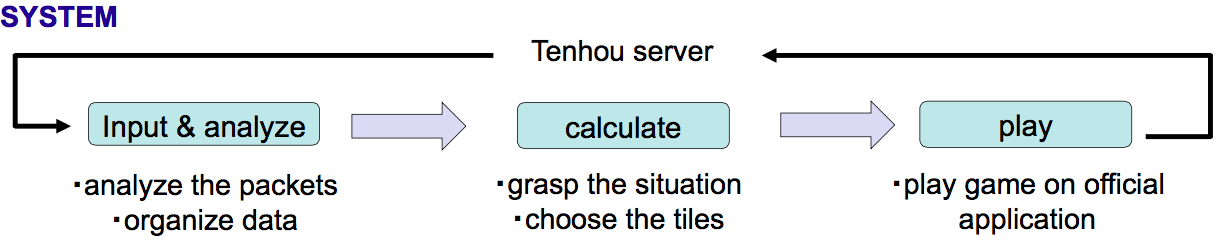
\includegraphics[keepaspectratio, scale=0.4
 ,bb=0 0 1226 243]
      {img/imp1.png}
 \caption{天鳳上で自動打ちするためのシステムの設計図}
 \label{imp1}
\end{figure}

まず、天鳳サーバーから受け取った情報を送られてくるパケットとして読み取る。次に、受け取った情報を整理・計算し選択する打牌を決定する。最後に、決定した打牌を公式アプリケーションを通じて天鳳サーバーにまた送るといった流れである。次の節以降その詳細について解説する。

\subsection{オンライン麻雀サイト天鳳}
天鳳は、現在インターネット上で麻雀を打つことができるサイトの中で最も利用者が多いサイトであり、登録者は390万人を超える大型のサイトである。また、アクティブユーザー(180日以内の対戦履歴があるプレーヤ数)は27万人を超え、現在最も活気のあるインターネット上の麻雀フィールドである。天鳳では麻雀研究に対する支援が充実しているという面も大きい。
最高ランク者のみが打つことのできる鳳凰卓というクラスの試合データ(以下牌譜)を全て公開しており、より良質な強者の牌譜を取得することができる。これらの牌譜は一日に約500試合ほど手に入り、量ともに十分利用できる。これについては、筆者も強者の統計的な手順について研究する際によく利用させていただいた。また、天鳳ではAIで麻雀を打つことを一定の条件下で許可している点も大きい。鳳凰卓については人間同士の生粋の強者のフィールドというコンセプトがあるため許可されていないが、その下の特上卓以下では条件を揃えることで対戦することが可能である。
一番下の一般卓については、最も低ランクなため対戦人数も多いため、AIによる影響が少ないと考えられている。そのためある程度対戦が可能なAIであれば、他プレイヤーの迷惑にならないような範囲での利用が許可されている。また、一般卓と鳳凰卓の間の上級卓・特上卓では、AIを用いて他のプレイヤーの不正検出に協力するという条件を元にAIの稼働を許可されている。AIを稼働させることによる他プレイヤーのメリットを提供することで、反対するものが少なくなるからである。本研究のシステムは、一般卓で稼働させた。

\begin{table}[h]
  \caption{ランク別リスト・AI稼働条件}
  \label{tb:rate2231}
  \begin{center}
  \begin{tabular}{c|c|c|c|c}
    \hline
    卓 & 一般卓   & 上級卓 & 特上卓 & 鳳凰卓\\\hline\hline
    レベル & 下位約80\% & 上位約20\% & 上位約10\% & 上位約1\% \\\hline
    AI稼働条件 & マナー厳守 & 不正検出に協力 & 不正検出に協力 & 不可\\\hline
  \end{tabular}\end{center}
\end{table}

% \subsection{プレイさせた天鳳のルール}
% ・ルールフロー図
% ・・天鳳上の制約(ルール)
% ・天鳳上の制約(マシン上の問題 持ち時間)

\subsection{入力}
天鳳サーバーから送られてくる情報を読み取るためには、プレイするための公式アプリケーションを扱う必要がある。天鳳では未だにAIを動かすための公式APIが公開されていないので、公式アプリケーションでプレイした情報を画像認識して解析するか、送られてくるパケットを解析する必要がある。本研究では、kmo2氏が公開している天鳳パケット解析用オープンソース\cite{kmo2}を利用し、パケット解析を利用することで情報の入力を行った。

\subsection{計算}
・天鳳からの情報をどういうふうな構造体で保存しているかどうかとか。

% \begin{figure}[h]
%  \centering
%  \includegraphics[keepaspectratio, scale=0.1,bb=0 0 3024 4032]
%       {img/flow.jpg}
%  \caption{4人麻雀自動打ちシステムのフローチャート}
% \end{figure}

また、シャンテン数の計算方法については、バックトラック法を用いた。バックトラック法とは、8クイーン問題の解決法で良くあげられるように、難しい組み合わせの問題を効率よく解くために考案された方法である。麻雀においては、シャンテン数を求めることはすなわち決められた牌姿を要素ごとの組み合わせに分解することであり、バックトラック法が有用である。雀頭・メンツ・ターツの組み合わせを最もシャンテン数を下げる形で分解することが必要になる。麻雀の和了形においては、雀頭が一つであるため、まずは雀頭として考えられる要素を取り出す。次に、メンツとして考えられる要素を取り出し、最後にターツを取り出す。メンツはターツからシャンテン数を一つ下げた形であるため、メンツで取り出せる部分がある場合はそちらを優先して行う。このようにして各要素の優先順位を付けながら考えられる組み合わせを抽出したとき、最もシャンテン数が小さいものがその牌姿のシャンテン数である。

\begin{figure}[h]
 \centering
 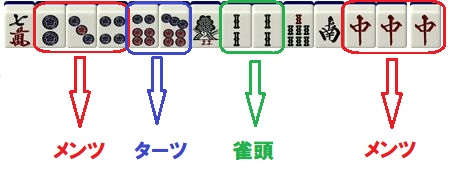
\includegraphics[keepaspectratio, scale=1,bb=0 0 320 220]
      {img/back.jpg}
 \caption{シャンテン数を求めるバックトラック法}
 \label{zu}
\end{figure}

\subsection{出力}
計算過程によって決定した牌を、天鳳サーバーに送信するためにも、プレイ用の公式アプリケーションを用いる。公式アプリケーションを介さないで直接データを送ることは、少しでも不正なプレイにならないようにするために必要なことである。公式アプリケーションで打牌を行うためには、決定した打牌をGUIで操作して選択する必要がある。したがって、出力過程では選択した牌をクリックできるよう、マウスイベントを呼ぶプログラム実装した。天鳳において公式アプリケーションで自動理牌を行うと、マンズ、ピンズ、ソーズ、字牌の順番になる。そのため、手牌の情報から切りたい牌が手牌の左から何番目にあるかを計算することができる。これを利用して、予め手牌の左端の座標を記憶し、そこから切りたい牌がどれだけ右側にあるかを計算させて、擬似的に切りたい牌を切るように設計した。


  % 本文4
\chapter{評価}
\label{chap:evaluation}
\section{1人麻雀における成績の評価}
提案手法で提示した、期待和了順目の評価による打牌選択のアルゴリズムを1人麻雀に適用し、性能を評価した。
図\ref{1houra}に示すのは、同じ5000局のテストデータを与え、対局を行うごとに和了率を測定し更新していったときのグラフである。また、天鳳において実力が上位0.1%に当たる上級者(本論文執筆者)と、天鳳において全体の50%に当たる平均プレイヤーを一人ずつ用意し、100局のテストデータで同じく和了率を比較した。\ref{100houra}この場合も同じテストデータで100局他のアルゴリズムによる和了率も測定している。図に示す「シャンテン数」のアルゴリズムとは、シャンテン数が最も少なくなるような牌を選択して打牌するアルゴリズムで、そのような牌が複数存在する場合はその中から切る。「有効牌」のアルゴリズムは、「シャンテン数」のアルゴリズムの中で、複数の牌が存在するときにその有効牌の枚数を比較して多いものを切るアルゴリズムである。最後に、「期待和了巡目」とあるアルゴリズムは、本研究で提案した、期待和了巡目の最も小さいものを選択するアルゴリズムである。


\begin{figure}[h]
 \centering
 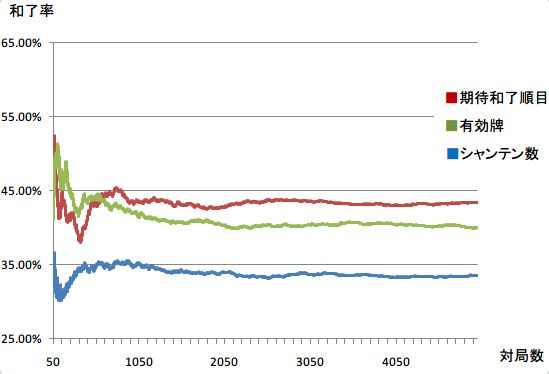
\includegraphics[keepaspectratio, scale=0.8,bb=0 0 549 374]
      {img/1houra.jpg}
 \caption{1人麻雀の和了率遷移}
 \label{1houra}
\end{figure}

\begin{table}[h]
  \caption{100局のデータセットでの和了率}
  \label{100houra}
  \begin{center}
  \begin{tabular}{c|c}
    \hline
    手法   & あがった局数(\%)\\\hline\hline
    上級者 	& 53 \\\hline
    期待和了巡目 & 44 \\\hline
    有効牌 	& 41 \\\hline
    平均プレイヤ 	& 36\\\hline
    シャンテン数	& 32 \\\hline
  \end{tabular}\end{center}
\end{table}

1人麻雀を5000局打たせたことによる和了率の比較では、「シャンテン数」<「有効牌」<「期待和了巡目」という結果となった。これは統計的に優位な水準での優劣である。結果については期待通りで、シャンテン数を下げるだけのアルゴリズムに対し、それをさらに有効牌の数を比べるアルゴリズムでは和了率が上昇した。また、本研究で提案した「期待和了巡目」のアルゴリズムでは、さらに有効牌の中でもより和了までの到達度を正確に計算することで和了率が上がることが確認された。1人麻雀による対局では、多人数性が存在しないため、本手法がうまく適用できると考えられる。また、上級者と平均実力者の人間プレイヤーを加えた100局の対局では、期待和了巡目のアルゴリズムの和了率は平均プレイヤーより優り、上級者に劣る結果となった。これは、上級者の場合はシャンテン数が瞬間的にあえて最小でないような打牌をして結果的に和了率がもっとも高くなる場合が存在するからであると考えられる。期待和了巡目はシャンテン数が最小になる牌の中から打牌を選択しているため、このような選択が行えない。
% \subsection{期待平均和了順目の探索の深さの評価}
% \subsection{モンテカルロ法の探索領域}


\section{4人麻雀における成績の評価} %麻雀サーバーとの対戦
本研究では1人麻雀における和了率の上昇を目指すため、静的指数である期待和了巡目を利用し、打牌を決定するアルゴリズムを提案した。これを第4章で設計した実装を元に、オンライン麻雀天鳳で打たせ、その成績を集計した。対戦した場所は天鳳の一般卓で、ルールは喰いアリ赤アリの東風戦、持ち時間は3秒である。2016年11月から2017年1月までの期間対戦を行い、試合数は2231戦となった。同じように、関連研究では1人麻雀のアルゴリズムを4人麻雀に適用し、実際の対人戦でその成績を評価している例が存在する。この節では、それらの研究の成績と本手法の比較を行い、その優位性を評価した。

評価として、和了率、放銃率、レーティングを比較した。


\subsection{和了率}
4人麻雀で実装した自動打ちシステムを対戦させた結果の、和了率の遷移を図\ref{houra2231}に示す。
50戦以下の対局では母数が少ないために和了率の偏差が大きいため、図は50戦以上の対局からの和了率を掲載した。和了率は300戦までは偏差が大きかったが、500戦を超えると徐々に収束していき、2231戦後の最終和了率は21.290%となった。

\begin{figure}[h]
 \centering
 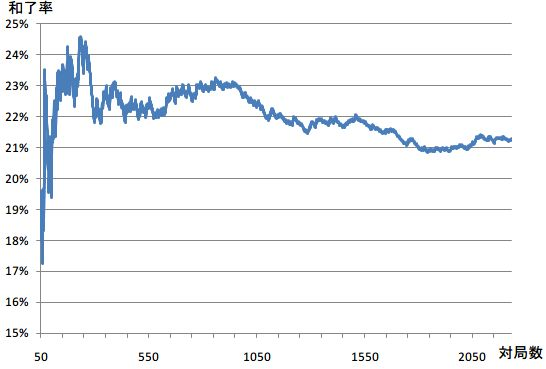
\includegraphics[keepaspectratio, scale=0.8,bb=0 0 546 369]
      {img/houra2231.jpg}
 \caption{和了率遷移}
 \label{houra2231}
\end{figure}

また、関連研究と比べた結果の表\ref{tb:houraritu}に示す。
佐藤らは有効牌を数え上げることによって打牌を選択するアルゴリズムを使用したが、その中で再帰の深さを変えたりヒューリスティックを加えたり複数の手法においてのデータを取っている。ただしそれらによる差は統計的に優位なほど大きな差ではなかったため、今回はそれらの中で最も基本的である再帰の深さ1のものと比較した。また、表にある平均プレイヤーとは、天鳳において平均レートが1500付近である初段のプレイヤーとした。そのデータは天鳳のランキングページに公開されているものを引用した。

\begin{table}[h]
  \caption{4人麻雀においての和了率の比較}
  \label{tb:houraritu}
  \begin{center}
  \begin{tabular}{c|c|c|c|c}
    \hline
    プレイヤー   & 本研究 & 佐藤らの研究 & 水上らの研究 & 平均プレイヤー\\\hline\hline
    対局数   & 2231 & 2526 & 504 & -\\\hline
    和了率(\%) & 21.3 & 20.1 & 18.8 & 21.9\\\hline
  \end{tabular}\end{center}
\end{table}

和了率を比較すると、本手法は佐藤らの研究をわずかに上回る結果となった。佐藤らの研究では有効牌の数え上げによって打牌を選択しているが、本手法では平均和了巡目を用いることでより先の展開を考慮した打牌の選択が可能になっていると考えられる。これは事前に期待されていたとおりであった。しかし、大きな差が生まれたというわけではなく、平均プレイヤーを優位に超えることはできなかった。これは、平均プレイヤーは鳴きによる和了も含まれているためであると考えられる。その理由に、1人麻雀による和了率(鳴きを含まない)は平均プレイヤーを超えていることがあげられる。ただし、4人麻雀でこれ以上の和了率を挙げるためには、やはり鳴きについての和了を加えないと難しいこともわかる。


\subsection{放銃率}
次に、和了率の遷移を図\ref{houra2231}に示す。
50戦以下の対局では母数が少ないために放銃率の偏差が大きいため、図は50戦以上の対局からの宝珠率を掲載した。放銃率は500戦までは下降を続けたが、1000戦を超えると徐々に収束していき、2231戦後の最終放銃率は18.377%となった。
\begin{figure}[h]
 \centering
 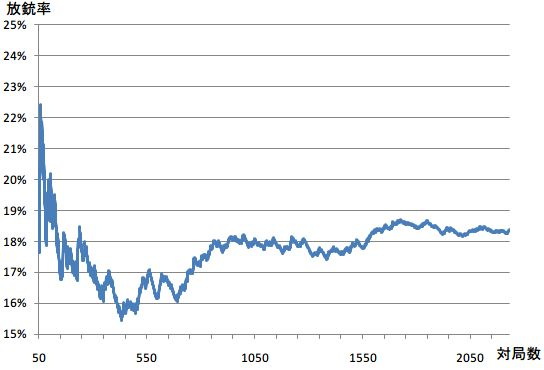
\includegraphics[keepaspectratio, scale=0.8,bb=0 0 544 370]
      {img/houzyu2231.jpg}
 \caption{放銃率遷移}
 \label{houzyu2231}
\end{figure}

また、関連研究と比べた結果を表\ref{tb:houzyu2231}に示す。
放銃率においてはどの研究にも大きな差は見られなかった。これらの研究では、4人麻雀におけるオリの戦略を加えていないからであると考えられる。平均プレイヤーはオリを行っているため、放銃率が低い。4人麻雀においては放銃率による失点は成績を悪くするため、重要な指標であるが、これらはオリの戦略を実装することで改善する必要があると考えられる。

\begin{table}[h]
  \caption{4人麻雀においての放銃率の比較}
  \label{tb:houzyu2231}
  \begin{center}
  \begin{tabular}{c|c|c|c|c}
    \hline
    プレイヤー   & 本研究 & 佐藤らの研究 & 水上らの研究 & 平均プレイヤー\\\hline\hline
    対局数   & 2231 & 2526 & 504 & - \\\hline
    放銃率(\%) & 18.4 & 18.9 & 19.0 & 16.4\\\hline
  \end{tabular}\end{center}
\end{table}

\subsection{レーティング}
レーティングとは、特定のプレイヤーが他のプレイヤーと比較してどの程度成績が良いかを図る評価の仕方の一つである。
レーティングは、平均順位と負の相関を持ち、式\ref{rate}で計算される。ゲームを行ったときの卓の平均のレーティングを$R_ave$とし、ゲームの結果の順位を$Rank$、ゲームを行う前のレーティングを$R$とした時、そのゲームによって更新されるレーティングがR'である。初期の時点でのレーティング($R$)は1500である。
\begin{equation}
\label{rate}
\Large R' = R + (50 - Rank × 20 + \displaystyle \frac{R_ave - R}{40} ) × 0.2
\end{equation}

4人麻雀で実装した自動打ちシステムを対戦させた結果の、レーティングの遷移を図\ref{rate2231}に示す。
50戦以下の対局では母数が少ないためにレーティングの偏差が大きいため、図は50戦以上の対局からのレーティングを掲載した。レーティングは500戦までは偏差が大きかったが、1000戦を超えると徐々に収束していき、2231戦後の最終放銃率は1382となった。

\begin{figure}[h]
 \centering
 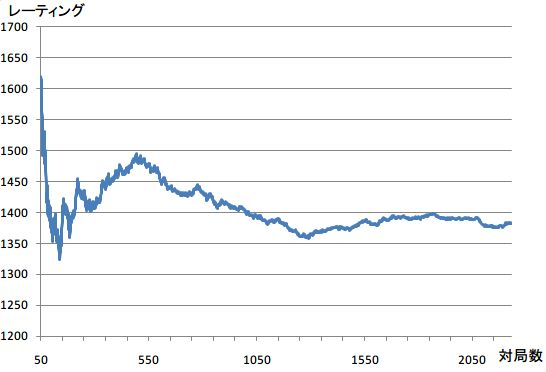
\includegraphics[keepaspectratio, scale=0.8,bb=0 0 546 372]
      {img/rate2231.jpg}
 \caption{レーティング遷移}
 \label{rate2231}
\end{figure}

また、関連研究と比べた結果を表\ref{tb:rate2231}に示す。
レーティングは佐藤らの研究をわずかに上回るという結果になった。しかし大きな有意差は見られず、平均プレイヤーにも及ばなかった。これは和了率の観点では本研究が優位なものの、四人麻雀では多人数性の理由によりほかの影響が多いことが考えられる。理由としては、1人麻雀では和了率が本研究の方が高いものの、放銃率では平均プレイヤーが低く出ているため、オリの影響が大きいと思われるからである。

\begin{table}[h]
  \caption{4人麻雀においてのレーティングの比較}
  \label{tb:rate2231}
  \begin{center}
  \begin{tabular}{c|c|c|c}
    \hline
    プレイヤー   & 本研究 & 佐藤らの研究 & 平均プレイヤー\\\hline\hline
    対局数   & 2231 & 2526 & - \\\hline
    レート & 1382 & 1339 & 1558\\\hline
  \end{tabular}\end{center}
\end{table}

% このように、レートは本手法の方が上回る結果となった。ここで保証安定レートについて比較をする。



  % 本文4
\chapter{結論}
\label{chap:conclusion}
\section{本研究のまとめ}
本研究では、各牌姿における期待和了巡目という途中局面の静的指数を評価することで、適切な打牌を選択するアルゴリズムを提案した。
評価として、1人麻雀における和了率、4人麻雀における和了率・放銃率・レーティングを比較した。
% 先行研究では UCB 1や LinUCB を1人麻雀に適用する例が報告されていたが、こ
% れらは和了までのシミュレーションを行っているものであり、探索空間が多く精度が落ちるため
% 平均プレイヤには及ばなかった。
本研究の提案手法では、1人麻雀の和了率が「シャンテン数を下げるように打つアルゴリズム」と「有効牌が多くなるように打つアルゴリズム」と比較して高いということが示された。また、平均プレイヤーよりも高い和了率であることが確認された。一方4人麻雀では、本研究の期待和了巡目を扱ったアルゴリズムが有効牌を扱ったアルゴリズムより和了率とレーティングがわずかに高いことが示された。しかし、大きな有意差は無く、どちらも平均プレイヤーに及ばなかった。

\section{本研究の結論}
1人麻雀における和了率の結果から、本研究の期待和了巡目を扱った打牌選択のアルゴリズムは面前の打牌選択において有用であることがわかった。麻雀において和了率が高いことは成績において重要であるため、その観点から麻雀の成績を上げることに利用できる可能性が高いということがわかった。しかし、4人麻雀においての和了率やレーティングの結果から、多人数性が存在する鳴きやオリの観点の考慮を行わないとこれ以上の成績向上が難しいことも確認できた。

% 本稿では, 牌譜の局面からの教師あり学習や異なる探索 の結果の共有ができる LinUCB を 1 人麻雀に適用すること を提案した. LinUCB と, 比較手法として UCB1 と事前学 習を利用する手法を 1 人麻雀に適用し, あがった局数を比 較することで評価を行った. その結果いずれの手法も人間 のプレイヤには及ばず, 3 つの手法では UCB1 が最も良い あがり率を出す結果となった. しかし, UCB1 と事前学習 のみを用いる手法の性能が近かったことから, 事前学習が 不完全情報ゲームに対してある程度有効であるということ が分かった. また, Plain LinUCB, 事前学習+LinUCB の 結果から特徴量の設計が不適切であったことが考えられる.
% 今後は特徴量の見直して実験を行い, LinUCB の性能評 価を再度行いたい. 本実験では, LinUCB と事前学習を利用 する手法を分けて評価を行ったが, LinUCB で成果が出る ようになれば, これらを組み合わせることで更に性能が向 上することが期待されるのでこれについても評価を行いた い. また, UCB をモンテカルロ木探索に適用した UCT [8] が成果をあげていることから LinUCB をモンテカルロ木探 索へ適用することも検討している.
\section{今後の課題と展望}
今回の検証で、1人麻雀の和了率において期待和了巡目を扱った方法はある程度の有用性を示すことが出来たが、上級者には及んでいない。この原因としては、期待平均和了順目を用いる方法では、ツモを無限試行回数行える場合の平均順目を最小にするように考えていることである。実際の1人麻雀では、ツモ回数が限られている。したがって、今後の課題としては、残りのツモ回数を考慮した期待和了巡目を考えることが必要になる。また、上級者と本研究の手法の違いには、変化を考慮するかしないかという点があげられる。上級者はシャンテン数が小さくなる選択肢があったとしても、敢えて長期的な目線でシャンテン数を増やさない選択を行う事がある。本研究においての期待和了順目はこのような変化を考慮していないが、これを考慮することでより高い和了率を出すことができる可能性があると考えられる。  % 本文5
% \chapter{映像伝送システム}
\label{chap:video-transmission}
\section{ビデオカメラ}
\section{ディスプレイ}
\section{インターレース}
\section{色空間}

映像では一般的に、RGBやYUV, YCbCr, YPbPrといった色空間で表現される。
色差成分を間引くことにより、

\section{帯域}

帯域は次のようになる。

表は次のように出力される(表\ref{tb:video-bandwidth})。

\begin{table}[htbp]
  \caption{表の例}
  \label{tb:video-bandwidth}
  \begin{center}
  \begin{tabular}{l|c|r|l|l}
    \hline
    解像度&フレームレート&色空間&ピクセルあたりのビット数&帯域\\\hline\hline
    3840x2160&60P&RGB&X bit&XX Gbps\\\hline
    3840x2160&30P&RGB&X bit&XX Gbps\\\hline
    3840x2160&30P&RGB&X bit&XX Gbps\\\hline
    3840x2160&30P&YUV 444&X bit&XX Gbps\\\hline
    3840x2160&30P&YUV 422&X bit&XX Gbps\\\hline
    3840x2160&30P&YUV 420&X bit&XX Gbps\\\hline
    1920x1080&60P&RGB&X bit&XX Gbps\\\hline
    1920x1080&60P&YUV&X bit&XX Gbps\\\hline
    1920x1080&30P&RGB&X bit&XX Gbps\\\hline
  \end{tabular}\end{center}
\end{table}


\section{インターフェース}
\subsection{HDMI 1.4/2.0}
\section{伝送手法}
\section{まとめ}

\chapter{ネットワークを活用した映像伝送}
\label{chap:network-transmission}
\section{仮説}
\subsection{Ethernetを活用するメリット}
\section{目的}
\section{構成}
\section{関連研究}

\chapter{システムの設計・実装}
\label{chap:implementation}
\section{UoIP} % UHD over IP
\section{システム構成}
\section{ソフトウェアによる実装}
\section{ハードウェアによる実装}
\subsection{FPGAの回路設計}

\chapter{評価}
\label{chap:evaluation}
\section{評価手法}
\section{計測}
\subsection{トラフィック}
\subsection{遅延}
\subsection{重量}
\section{考察}

\chapter{結論}
\label{chap:conclusion}
\section{本研究のまとめ}
\section{今後の課題と展望}

citation\cite{hoge09}
  % 仮

\begin{acknowledgment}

このテンプレートを改造するにあたって、@kurokoboとインターネット上のいくつかの修士論文などを参考にしました。感謝いたします。

\end{acknowledgment}
  % 謝辞。要独自コマンド、include先参照のこと

\begin{bib}[100]
% BibTeXを使う場合
\bibliography{bib/main}

%\begin{thebibliography}{#1}
%
%  \bibitem{参照用名称}
%    著者名:
%    \newblock 文献名,
%    \newblock 書誌情報,出版年.
%
% \bibitem{hoge09}
%   ほげ山太郎,ほげ山次郎:
%   \newblock ほげほげ理論のHCI分野への応用,
%   \newblock ほげほげ学会論文誌,Vol.31,No.3,pp.194-201,2009.
%
% \bibitem{hoge08}
%   Taro Hogeyama, Jiro Hogeyama:
%   \newblock The Theory of Hoge,
%   \newblock {\it The Proceedings of The Hoge Society}, 2008.
%
%\end{thebibliography}

\end{bib}
  % 参考文献。要独自コマンド、include先参照のこと

\appendix
% \chapter{付録の例}

付録を無理矢理出力させるため、てきとうなことを書く。

\section{ほげ}

コマンドは本文と一緒。

\subsection{ふー}

本文と一緒。

\section{ほげほげ}

本文と一緒。

\subsection{ふーふー}

本文と一緒。
    % 付録

\end{document}
